\documentclass[a4paper,11pt] {article}
\usepackage[spanish]{babel}
\usepackage[utf8]{inputenc}
\usepackage{caratula}
\usepackage{a4wide}
\usepackage{graphicx}
% \usepackage{dot2texi}
% \usepackage{graphs}

\begin{document}

\titulo{Trabajo Pr\'actico Nro. 3}
\fecha{08/05/2009}
\materia{Algoritmos y Estructuras de Datos III}
\grupo{}
\integrante{Dinota, Mat\'ias}{076/07}{matiasgd@gmail.com}
\integrante{Huel, Federico Ariel}{329/07}{federico.huel@gmail.com}
\integrante{Leveroni, Luciano}{360/07}{lucianolev@gmail.com}
\integrante{Mosteiro, Agust\'in}{125/07}{agustinmosteiro@gmail.com}

\maketitle

\bigskip
\section*{Aclaraciones generales}

Antes de comenzar el an\'alisis de cada ejercicio, cabe mencionar lo siguiente:

\begin{itemize}
 \item La implementaci\'on de los 3 algoritmos se realiz\'o en \textbf{lenguaje Java}, haciendo uso de las librer\'ias est\'andar del mismo.
 \item Para el c\'alculo de tiempo de los algoritmos se utiliz\'o la funci\'on \textbf{nanoTime()} de la clase System de Java. Con el fin de aumentar la precisi\'on de las mediciones, se utiliz\'o el comando \textbf{nice} para darle m\'axima prioridad a la tarea.
 \item El c\'odigo fuente de los algoritmos aqu\'i analizados se encuentran en los archivos \textit{Dengue.java} (Ej 1), \textit{Diamante.java} (Ej 2) y \textit{RedAstor.java} (Ej 3).
 \item El c\'odigo fuente de los programas encargados de hacer uso de los algoritmos y necesarios para compilar las aplicaciones son:
 \begin{itemize}
    \item \underline{Ej 1:} MainDengue.java, Dengue.java e InstanciaDengue.java.
    \item \underline{Ej 2:} MainDiamante.java, Diamante.java, InstanciaDiamante.java.
    \item \underline{Ej 3:} MainRedAstor.java, RedAstor.java, InstanciaRedAstor.java, Arista.java, AristaComparator.java, Dupla.java, DuplaComparator.java.
  \end{itemize}
 \item Para la lectura y escritura de los datos se utilizaron clases provistas por el lenguaje Java. No se har\'a referencia a estos algoritmos ya que no resultan de inter\'es para el trabajo aqu\'i presentado.
 \item Los gr\'aficos se realizaron con \textbf{GNUPlot} y Calc. En los casos considerados pertinentes, se utiliz\'o una escala logar\'itmica con el fin de poder visualizar mejor los resultados.
\end{itemize}

%EXPLICAR LO DE LAS DENSIDADES!!!!!

\begin{center}
\section*{Introducci\'on}
\end{center}

El objetivo del siguiente trabajo es presentar diversos m\'etodos para encontrar soluciones exactas y aproximadas para el problema del Conjunto Independiente de Peso M\'aximo (CIPM). En particular, se desarrollar\'a un algoritmo que utiliza la t\'ecnica de \textit{backtracking} para resolver el problema de manera exacta para instancias peque\~{n}as del mismo. Adem\'as, se implementar\'an heur\'isitcas constructivas, de b\'usqueda local y una metaheur\'istica GRASP, la cual ser\'a el foco principal de nuestro estudio.

Para cada tipo de heur\'istica (constructivas y de b\'usqueda local), se realizar\'an pruebas para determinar cual es la m\'as eficaz y, en caso de ser posible, cu\'al es la m\'as precisa en relaci\'on a la soluci\'on exacta del problema. En estas decisiones tambi\'en se tendr\'a en cuenta el tiempo de ejecuci\'on de cada una las heur\'isticas, procurando obtener un balance entre eficacia de la soluc\'on y tiempo de ejecuci\'on.

Finalmente, se desarrollar\'a una metaheur\'istica GRASP modificando ligeramente las heur\'isticas constructivas y de b\'usqueda local previamente mencionadas. Se realizar\'an pruebas para determinar con cuales de estas heur\'isticas la soluci\'on de GRASP es m\'as precisa. Tambi\'en se har\'an estudios sobre la eficacia de la soluci\'on en relaci\'on a los par\'ametros involucrados en esta metaheur\'istica. A partir de estos resultados se podr\'an concluir los par\'ametros adecuados y las heur\'isticas a utilizar para que el resultado de GRASP sea eficaz y eficiente en relaci\'on al tiempo de ejecuci\'on.

Por \'ultimo, para la metaheur\'istica GRASP obtenida y para las mejores heur\'isticas (constructiva y de b\'usqueda local) se mostrar\'an casos en donde el resultado de las mismas difiera del exacto en gran medida. Adem\'as, se estudiar\'a la complejidad te\'orica de estos algoritmos y se realizar\'an comparaciones con el tiempo de ejecuci\'on obtenido en las pruebas.

\section*{Algoritmo Exacto}

En primer lugar, nos ocuparemos del análisis de un algoritmo exacto propuesto para resolver el problema en cuestión. A continuación, se presenta el pseudocódigo que esboza el comportamiento del mismo:

\begin{verbatim}
para cada nodo (nodoActual) del grafo
    apilar nodoActual
    mientras la pila no sea vacia
        para cada nodo desde nodoActual+1 en adelante
            si ese nodo no es adyacente a ninguno de la pila
                apilar nodo
        finPara
        si la suma de pesos de los nodos de la pila > peso de la solucion
            solucion = pila
        nodoActual = desapilar nodo
    finMientras
finPara
\end{verbatim}

Como se puede observar, el algoritmo utiliza la técnica de \textit{backtracking} para resolver el problema. La idea general del mismo consiste en observar todos conjuntos independientes (CI) de cada subgrafo $S$ de G inducido por los nodos desde un nodo $i$ hasta $n$ que contengan al nodo $i$, para $1 \leq i \leq n$\footnotemark[1]. Cada iteración del ciclo externo del algoritmo se encargará de buscar todos los CI para cada uno de los subgrafos.

Antes de continuar, es importante notar que esto garantiza encontrar el conjunto independiente de peso máximo de $G$. La demostración es simple: Sea $j$ el nodo mínimo del CI de peso máximo del grafo $G$. Como en cada iteración $i$, el algoritmo busca todos los conjuntos independientes que contengan al nodo $i$ en S, con $i$ desde $1$ hasta $n$, entonces existe una iteración del algoritmo donde $i = j$. En dicha iteración, por hipótesis, se observan todos los conjuntos independientes que están compuestos por $j$ y nodos mayores a $j$, y como $j$ es el nodo mínimo de la solución, uno de esos conjuntos deberá ser dicha solución.

A continuación, se mostrará como en cada iteración del ciclo externo, el algoritmo observa los CI de los subgrafos S mencionados.

El ciclo utiliza una pila que comienza conteniendo únicamente al nodo $i$. Luego, se van agregando todos los nodos que vayan conformando un conjunto independiente apartir de ese nodo \textit{i} hasta el último del grafo.
Inmediatamente después, en caso de que dicho conjunto independiente sea el de peso máximo\footnotemark[2] hasta el momento, se almacena la pila como solución. El siguente paso consiste en desapilar el tope de la pila (que contiene al último nodo insertado), observando si cada nodo posterior a éste puede ser apilado de modo que se siga manteniendo el invariante de conjunto independiente, es decir, se insertan los nodos que no sean adyacentes a \underline{ningún} nodo de la pila. De esta manera, al salir del ciclo, se habrán observado todos conjuntos independientes que contengan al nodo $i$, ya que es condición del ciclo que dicho nodo esté en la pila por ser el primer nodo apilado.

Por todo esto, podemos afirmar que el algoritmo encontrará el conjunto independiente de peso máximo para cualquier grafo G.

\footnotetext[1]{Recordemos que cada nodo del grafo está numerado desde 1 hasta $n$.}
\footnotemark[2]{Dicho peso se encuentra ya almacenado en simple acumulador.}

\section*{Complejidad}

En la presente secci\'on se calcular\'a la complejidad en el peor caso del algoritmo exacto presentado para resolver el problema. Como se mostr\'o en anteriores secciones, para un grafo $G$ el algoritmo, en cada iteraci\'on $i$, busca todos los conjuntos independientes formados por el nodo $i$ y todos los nodos mayores que $i$ en el subgrafo inducido por dichos nodos. El peor caso de este algoritmo ocurre cuando el grafo est\'a formado solamente por nodos aislados (grado 0). En este caso, el algoritmo deber\'a buscar todos los conjuntos posibles que se pueden formar a partir de los nodos del grafo ya que cualquier combinaci\'on de nodos forma un conjunto independiente. Como la cantidad de conjuntos posibles que se pueden formar con $n$ nodos es $2^{n}-1$, se deduce que la complejidad en el peor caso ser\'a $O(2^{n})$. Sin embargo, en casos donde la cantidad de aristas sea mayor, la cantidad de conjuntos independientes que deber\'a comprobar el algoritmo ser\'a mucho m\'as reducida. Evitando el chequeo de conjuntos innecesarios se espera que el tiempo de ejecuci\'on sea m\'as reducido para grafos con densidades altas, es decir, con gran cantidad de aristas.

\section*{An\'alisis de resultados}

El siguiente analisis est\'a orientado a estudiar el tiempo de ejecuci\'on del algoritmo exacto en relaci\'on a los datos de entrada (cantidad de nodos de los grafos), comparando el costo real del algoritmo junto con su complejidad te\'orica calculada. Como vimos anteriormente el m\'etodo exacto tiene una alta complejidad temporal por lo que, al momento de realizar las mediciones, se utilizaron grafos en los que su cantidad de nodos var\'ia entre 1 y 36.

En cuanto al tipo de grafos utilizados, se opt\'o por analizar el comportamiento del algoritmo sobre grafos con distintas densidades debido a que la cantidad de conjuntos independientes se modifica notablemente seg\'un este par\'ametro. De esta manera, para cada grafo de un mismo tama\~{n}o, se realizaron tres pruebas, variando entre altas, medias y bajas densidades.

Cabe mencionar que los grafos sobre los que se aplic\'o el algoritmo fueron generados aleatoriamente y que el tiempo de ejecuci\'on del mismo fue calculado mediante el uso de la funci\'on \textit{nanoTime()} de Java.

Los resultados arrojados fueron los siguientes:

\begin{center}
 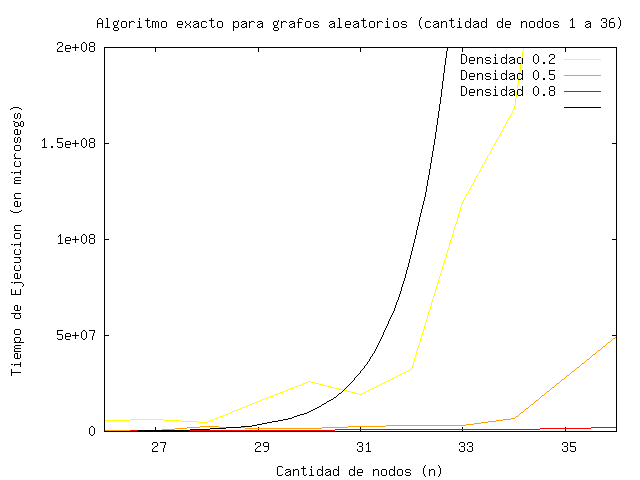
\includegraphics[width=0.9\textwidth]{graficos/tiemposExacto.png}
\begin{center}
Figura 1.1
\end{center}
\end{center}

Como se puede apreciar en el gr\'afico, el tiempo de ejecuci\'on del algoritmo aplicado sobre los distintos grafos seleccionados se comporta de acuerdo a la complejidad te\'orica estimada. Adem\'as, podemos ver que se mantiene muy alejado de la cota para el peor caso ($2^{n}$).

Otro aspecto a tener en cuenta es la notable diferencia de los tiempos en relaci\'on a las diversas densidades. Se puede ver que si la densidad del grafo es baja, el tiempo de busqueda del conjunto independiente de mayor peso es mucho mayor que si se lo busca sobre un grafo de densidad media. Lo mismo sucede entre media y alta densidad. Esto se debe a que al disminuir la cantidad de aristas (menor densidad), la cantidad de conjuntos independientes en el grafo aumenta, ya que mientras menos aristas haya, mayor cantidad de nodos no adyacentes entre si habr\'a. De esta manera, mientras menor sea la densidad, mayor ser\'a la cantidad de conjuntos independientes a tener en cuenta por el algoritmo con el fin de buscar el de mayor peso, por lo que demandar\'a mayor tiempo de ejecuci\'on.

\bigskip

\begin{center}
\section*{Heur\'isticas constructivas}
\end{center}

\section*{Esquema general}

A continuaci\'on se desarrolar\'a el trabajo realizado sobre heur\'isticas constructivas con el objetivo de reducir significativamente la complejidad temporal a merced de una p\'erdida de eficacia en las soluciones. Para esto, se utilizar\'on distintos algoritmos golosos que tienen en cuenta diversas condiciones sobre los nodos para ir armando una soluci\'on de manera constructiva. Se pensaron varias ideas para buscar aproximarse a la soluci\'on \'optima, todas siguiendo el siguiente esquema de algoritmo goloso:

\begin{verbatim}
mientras haya nodos en el grafo
  maxF = 0 | minF = n
  para cada nodo del grafo
    si grado(nodo) = 0
      agregar nodo a solucion
      borrar nodo del grafo
    sino
      si f(nodo) >= maxF | f(nodo) <= minF
        maxF | minF = f(nodo)
        nodoMax | nodoMin = nodo
  finPara

  agregar nodoMax a solucion
  borrar vecindad de nodoMax
\end{verbatim}

Podemos apreciar que en cada iteraci\'on (del ciclo interno) el algoritmo recorre todos los nodos verificando que se cumpla una condici\'on de acuerdo a una funci\'on aplicada a los mismos (funci\'on $f$). Una vez observados todos los nodos, se agrega el nodo m\'aximo o m\'inimo de acuerdo a la condicion mencionada al conjunto soluci\'on. De inmediato, se procede a borrar la vecindad de dicho nodo del grafo. De esta manera, en cada iteraci\'on, el grafo contendr\'a una cantidad cada vez menor de nodos de modo de garantizar que el algoritmo termina (sale del ciclo principal).

Cabe aclarar que si el grado de los nodos que el algoritmo va recorriendo es igual a 0, inmediatamente son agregados a la soluci\'on. Esto se debe a que, al ser todos los pesos mayores que 0, si un nodo no es adyacente a ning\'un otro (grado 0), siempre deber\'a pertenecer a la soluci\'on.

Las distintas funciones $f$ aplicadas sobre los nodos para armar el conjunto soluci\'on fueron:

\begin{itemize}
\item Peso: en cada iteraci\'on del algoritmo se agrega a la soluci\'on el nodo de mayor peso.
\item Grado: en cada iteraci\'on del algoritmo se agrega a la soluci\'on el nodo de menor grado. La idea de aplicar dicha funci\'on es que, al agregar a la soluci\'on el nodo de menor grado, solo se borrar\'an del grafo los nodos de su vecindad (que es la de menor tama\~{n}o) descartando asi la menor cantidad de nodos posible.
\item Peso/Grado: en cada iteraci\'on del algoritmo se agrega a la soluci\'on el nodo de mayor cociente peso/grado. Simplemente una combinaci\'on de las dos t\'ecnicas mencionadas anteriormente.
\item Peso/Vecindad: en cada iteraci\'on del algoritmo se agrega a la soluci\'on el nodo de mayor cociente peso*grado/pesoVecindad. La intenci\'on en este caso es ponderar tambi\'en el peso y la cantidad de nodos de la vecindad del nodo a agregar a la soluci\'on (si la vecindad del nodo es muy pesada y posee pocos nodos no quiero descartarla).
\end{itemize}

\section*{An\'alisis de eficacia de las heur\'isticas}

Con el objetivo de decidir que heur\'istica es m\'as eficaz en relaci\'on a la precisi\'on de la soluci\'on obtenida, se realizaron pruebas para 27 grafos distintos generados de manera aleatoria. En los casos que fue posible, se compar\'o el resultado obtenido con la soluci\'on exacta del problema, obtenida por medio del algoritmo exacto presentado anteriormente.

Los grafos generados de manera aleatoria se dividen en 3 tipos seg\'un la cantidad de nodos. Se crearon 9 grafos de cada tipo, con cantidad de nodos 30, 300 y 600. A su vez, cada tipo de grafo se divide seg\'un la densidad del grafo, es decir, de los 9 grafos de cada tipo se crearon 3 con baja, media y alta densidad. El peso de cada uno de los nodos tambi\'en es aleatorio, en un rango de 1 a $n*10$, siendo $n$ la cantidad de nodos. Estos grafos ser\'an utilizados en todas las pruebas que se realizar\'an en el trabajo, tanto para las heur\'isticas constructivas como para las b\'usquedas locales y la metaheur\'istica GRASP.\footnotemark[1]

Para cada uno de los grafos mencionados se ejecutaron todas las heur\'isticas constructivas mencionadas en la secci\'on anterior, obteniendo los siguientes resultados.

\begin{center}
 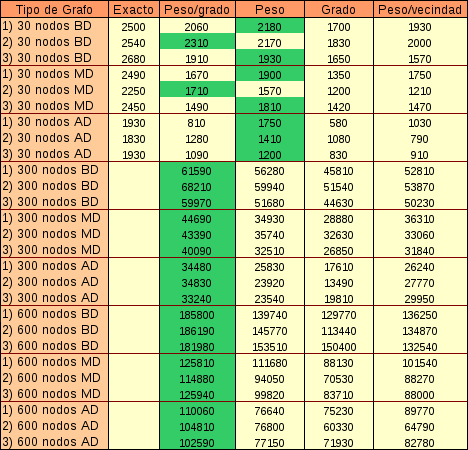
\includegraphics[width=0.75\textwidth]{tablas/tablaHC.png}
\begin{center}
Figura 2.1
\end{center}
\end{center}

Las pruebas realizadas a grafos de 30 nodos pueden ser comparadas con el resultado exacto obtenido por medio del algoritmo de \textit{backtracking}. Como se puede observar, todos los resultados de las heur\'isticas difieren del resultado exacto en distinta medida. Esto es un resultado esperable ya que en la mayor\'ia de los casos todas las heur\'isticas golosas no son eficaces y se pueden encontrar casos en los que el resultado difiera en gran medida del exacto.

En la tabla presentada fueron remarcados los resultados m\'as altos para cada tipo de grafo. Como se puede apreciar, para grafos con 30 nodos, los mejores resultados fueron obtenidos con la heur\'istica de Peso. Sin embargo, para grafos con mayor cantidad de nodos, como los de 300 y 600 nodos, los resultados de la heur\'istica de Peso/grado son ampliamente mejores.

A partir de estos resultados, se puede concluir que la heur\'istica de Peso/Grado es la m\'as eficaz de las heur\'isticas implementadas.  El fundamento m\'as importante para la elecci\'on de la misma fue que los resultados para grafos con gran cantidad de nodos, son mucho m\'as eficaces a las dem\'as heur\'isticas constructivas. Como las heur\'isiticas fueron pensadas para resolver instancias de tama\~{n}o mucho mayor a lo que el algoritmo exacto puede resolver, es razonable que se elija la heur\'istica que mejor se comporte para grafos con gran cantidad de nodos. Adem\'as, para grafos peque\~{n}os los resultados no difieren demasiado de los obtenidos con la heur\'istica de Peso.

En posteriores secciones estudiaremos el comportamiento de la heur\'istica Peso/grado en relaci\'on al tiempo de ejecuci\'on y compararemos dichos resultados con su complejidad te\'orica.

\section*{Complejidad}

Para calcular la complejidad de este ejercicio el modelo utilizado fue el uniforme, esto se debe a que lo que define el orden del algoritmo es la cantidad de nodos y de aristas (y cómo están relacionados los nodos  por dichas aristas). Teniendo en cuenta que los nodos van de 1 a $n$, no es relevante observar el tamaño que ocupa cada nodo, sino la cantidad de estos, ya que si el número que representa a un nodo es muy grande, igual de grande es la cantidad de nodos en el grafo y pierde sentido utilizar el modelo logarítmico.

\bigskip
Al crear las listas de adyacencias, el algoritmo lee $2m$ aristas del archivo de entrada y las agrega en dichas listas. Para esto crea n listas que representan las adyacencias de cada nodo. Como hay $2m$ aristas que se distribuirán en n listas(dónde la inserción es en $O(1)$), la complejidad temporal de realizar esta tarea será $O(2m + n)$.

Luego se filtran los nodos de grado 0 y 1. Aquí se recorren las listas de adyacencias y se eliminan los nodos que no tengan(en el grafo original) al menos dos nodos adyacentes. Esto requiere recorrer todas las listas de adyacencias que cuesta $2m + n$ (esto se debe a que para que un nodo sea adyacente a otro debe existir una arista y una arista no puede conectar a más de un nodo).

\begin{verbatim}
crear grafo representado por array de lista de adyacencias (llamado 'adyacencias')
excepto para los nodos de grado 1 y 0
\end{verbatim}

A partir de ahora llamamos $n$ a la cantidad de nodos que pertenecían al grafo y no fueron filtrados por su grado.
Dado esto, $sn$  està acotado por  $m$, ya que cada nodo tiene asociada por lo menos 2 aristas y como cada arista sòlo puede asociar a dos nodos, la mìnima cantidad de aristas es $n$. Entonces el costo de $n^2$ està acotado por $n*m$.

\bigskip

El costo de armar la matriz de adyacencias resulta de crear una matriz de $n^2$ posiciones con ceros y recorrer las listas de adyacencias y agregar en las 2 posiciones adecuadas en la matriz ($O(1)$) un 1. Entonces cuesta $n^2+m$. Al ser $n<m$, cuesta $n*m$.

\begin{verbatim}
armar la matriz de adyacencias de ese grafo
\end{verbatim}

Luego se crean las vecindades para los nodos con grado mayor o igual a 3 y se busca el diamante mínimo que exista en cada una de dichas vecindades.

\begin{verbatim}
para cada nodo (que llamaremos superNodo) del grafo
  si el tamaño de la lista de adyacencia de superNodo es mayor que 3
    crear la vecindad del superNodo (crearVecindad)
    buscar el diamante minimo de esa vecindad (buscarDiamanteMinimoEnVecindad)
    y agregarlo a diamantesMinimos (si es que hay alguno)
\end{verbatim}

Creación de la vecindad para un nodo $i$:

Para cada nodo $k$ adyacente a $i$ se recorren sus adyacentes y se los agrega a una componente de la vecindad si el nodo es también adyacente a $i$.
Esto implica recorrer la lista de adyacencias de $i$ y ,para cada uno de sus  adyacentes, recorrer su lista de adyacencia. Como en una lista de adyacencias de un grafo no hay nodos repetidos, recorro como máximo una sola vez la lista de adyacencias de un nodo. A su vez, la cantidad de nodos contenidos entre todas las listas de adyacencias de un grafo es $2m$.

Luego, para crear la ‘vecindad’ de un nodo, se recorren como máximo $2m$ nodos con los cuales se verifica ,por cada uno, si dos son adyacentes ($O(1)$ en la matriz de adyacencia) y se los agrega a una lista ( $O(1)$ por agregarse al principio). Por lo que crear la ‘vecindad’ de un nodo es de orden $m$.

\begin{verbatim}
crearVecindad(superNodo)
  para cada nodo k de adyacencias[superNodo]
    para cada nodo j de adyacencias[k]
      si nodo j es adyacente a superNodo
        agregar nodo j a listaVecindad
    vecindadDeSuperNodo[k] = listaVecindad
  devolver vecindadDeSuperNodo (grafo representado por array de listas de adyacencia)
\end{verbatim}

Búsqueda del diamante mínimo en una determinada vecindad.

Para buscar el diamante mínimo en una vecindad lo que hace el algoritmo es recorrer por DFS cada componente conexa de la vecindad de un nodo,  sumando los grados de cada nodo, guardando los nodos y eligiendo el mínimo de ellos.
Para esto recorremos la vecindad agregando los nodos que van apareciendo en el camino a una pila si no fueron marcados (en un array, $O(1)$). Es decir que, una vez más, para cada nodo se revisa su lista de adyacencias. Esto es de orden $n + m$.

Si existe el diamante, se lo busca de la siguiente manera:

Para esto se calcula el nodo mínimo nodo, que no se relacione con todos los demás de la componente, es decir, se recorren a lo sumo $n$ nodos y se va guardando el menor, lo que cuesta a lo sumo $n$.
Luego para cada uno de sus adyacentes que pertencen a la vecindad de $i$, se recorre su lista de adyacencia (ya se mencionó antes que el costo de realizar esto es $m$) y se verifican adyacencias hasta encontrar los nodos que cumplan la condición de ser adyacentes a $i$, y no ser adyacentes entre sí.
Una vez encontrados estos nodos, se los ordena. Al ser cuatro nodos el tiempo es constante. 
Es decir que la complejidad de encontrar el diamante minimo en una determinada componente conexa es $O(n + m) = O(m)$

Como hay que crear la vecindad para cada uno de los nodos de grado mayor o igual a 3, el número de vecindades va a depender de la cantidad de nodos. Luego, si existe el diamante se lo busca en orden $m$.
Es decir que el orden de crear una vecindad ($n$) se sumará al de buscar su diamante si es que existe ($n$) por cada nodo estudiado. Luego, esto se realiza a lo sumo n veces, una vez por cada nodo.

Es decir que el costo de crear todas las vecindades y buscar su diamante es $n * m$.

\begin{verbatim}
buscarDiamanteMinimoEnVecindad(vecindadDeSuperNodo)
  recorrer cada componente conexa de vecindadDeSuperNodo por DFS
  sumando los grados de los nodos recorridos (sumaGradosCompConexa) y
  guardando en nodosCompConexa los nodos recorridos y
  en nodoMinimoCompConexa el nodo minimo de la componente conexa

  si sumaGradosCompConexa != a la cantidad de nodos
  del grafo completo de los nodos de la comp conexa
    si diamanteMinimo no existe
      diamanteMinimo = diamante minimo de comp conexa actual 
      (buscarDiamanteMinimoDeCompConexa)
    sino
      si nodoMinimoCompConexa <= el minimo nodo de diamanteMinimo
        diamante = diamante minimo de comp conexa actual 
        (buscarDiamanteMinimoDeCompConexa)
        si diamante existe y es mas chico que diamanteMinimo
          diamanteMinimo es ese diamente

  devolver diamanteMinimo (puede ser nulo en caso de que no haya diamante)

buscarDiamanteMinimoDeCompConexa(superNodo, vecindadDeSuperNodo, nodosCompConexa)
  nodo1 = superNodo
  nodoMinimo = nodo minimo de nodosCompConexa con grado menor 
  que cantidad de nodos de la componente conexa - 1

  tuplaMin = <nodo mas grande del grafo, nodo mas grande del grafo>
  para cada nodo (adyacenteANodo2) de vecindadDeSuperNodo[nodo2]
    para cada nodo (nodoCandidato) de vecindadDeSuperNodo[adyacenteANodo2]
      si nodoCandidato no es adyacente a nodo2 
      y <nodoCandidato, adyacenteANodo2> < tuplaMin
        tuplaMin = <nodoCandidato, adyacenteANodo2>

  nodo3 = primero(tuplaMin)
  nodo4 = segundo(tuplaMin)

  diamanteMinimo = ordenar(nodo1, nodo2, nodo3, nodo4)

  devuelvo diamanteMinimo

\end{verbatim}

Cuando ya se tienen los diamantes mínimos de cada vecindad, resta encontrar el mínimo de todos. Es importante notar que no puede haber más componentes conexas que nodos, ya que la componente conexca más chica tiene un nodo(más allá de que debe tener por lo menos cuatro nodos para que haya un diamante.

Como los diamantes tienen 4 nodos, se los compara componente a componente en $O(1)$ y se descarta el mayor de los dos hasta que sólo quede un diamante. Entonces se comparan a los sumo n diamantes en $O(1)$ por lo que en tiempo lineal se consigue el mínimo de los diamantes a partir de los diamantes mínimos de cada vecindad.

\begin{verbatim}
si hay algun diamante en diamantesMinimos retorno minimo(diamantesMinimos)
\end{verbatim}

Luego de haber analizado la complejidad del algoritmo en cada una de las partes (siendo éstas independientes entre si), se puede concluir que el orden del algoritmo en total será equivalente a la de mayor complejidad, es decir $O(n*m)$.

\bigskip

Finalmente estudiaremos la complejidad en funci\'on del tama\~{n}o de la entrada. Sea $t$ el tama\~{n}o de la entrada, $n$ la cantidad de nodos, y $m$ la cantidad de aristas. Tenemos entonces que:

$$t=2m+1\log(n)>m\log(n)$$

\hspace{45pt} $\Longrightarrow$ como $T(n,m) \in O(nm)$ y $nm<n^{m}=2^{m\log(n)}<2^{t} \Longrightarrow T(t) \in O(2^{t})$

\section*{An\'alisis de resultados}

Al igual que para el análisis del algoritmo exacto, se generaron grafos aleatorios con 3 tipos de densidades con el fin de evaluar el comportamiento de la heurística constructiva elegida sobre diversos grafos según la cantidad de nodos. Sin embargo, al tratarse de un algoritmo polinomial, la cantidad de nodos analizados será mucho mayor (desde 10 hasta 1400 nodos) con el fin de poder observar con claridad su comportamiento.

Como hemos visto anteriormente, la complejidad de la heurística constructiva resulta del orden $n*m$. Por este motivo, se han incluido en el gráfico las curvas $(n^2)/25$ y $(n^3)/15000$ con el fin de observar el comportamiento para grafos de distinta densidad. De esta manera, los tiempos de ejecución de grafos de alta densidad (donde $m$ tiene a $n^2$) deberían ser similar a la curva $(n^2)/25$ mientras que los de baja (donde $m$ tiene a $n$) deberían asimilarse a la curva $(n^2)/25$. A continuación, se presenta el gráfico en cuestión.

\begin{center}
 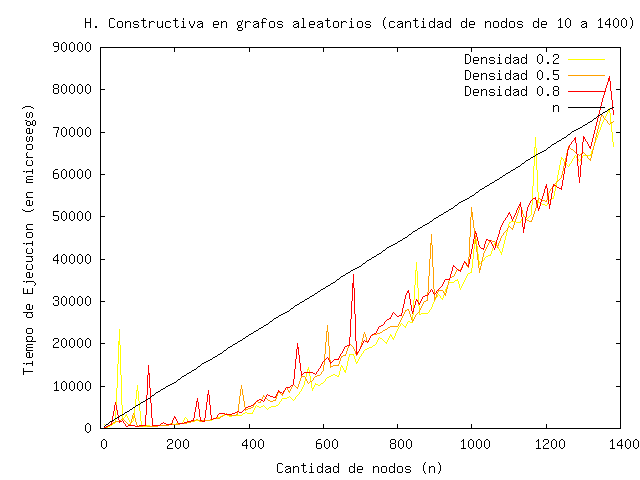
\includegraphics[width=0.7\textwidth]{graficos/tiemposHC.png}
\begin{center}
Figura 2.1
\end{center}
\end{center}

Como se observa, el comportamiento no es el esperado, ya que que para grafos de densidad variada, los tiempos de ejecución siempre se comportan de la forma de $n^2$, lo que haría suponer que la complejidad real del algoritmo podría ser $O(n^2)$. Sin embargo, este fenómeno podría tener relación con la conjetura realizada al haber conjeturado

\section*{Conclusiones}

En esta \'ultima secci\'on se realizar\'a una breve descripci\'on de los temas y resultados a tener en cuenta sobre este ejercicio. La primer parte del ejercicio requiri\'o un estudio profundo de teoria sobre subgrafos diamantes lo que permiti\'o una mayor facilidad para encarar la segunda parte y una buena cantidad de ideas a tener en cuenta. Sin embargo, el algoritmo presentado debi\'o encargarse de numerosas complicaciones que, a la hora de realizar la demostraci\'on de la propiedad referida al tema, no hab\'ian sido tenido en cuenta.

En mayor parte esto se debi\'o a la complejidad exigida por la c\'atedra lo que motiv\'o a la utilizaci\'on de distintas estructuras y m\'etodos (matrices y listas de adyacencia, estructuras de mapeo, algoritmos de busqueda inteligente, etc) que pudieran cumplir con lo pedido. Otro aspecto dificultoso fue el hecho de tener que retornar el diamante de menor tama\~{n}o, lo que implic\'o tener que guardar un registro de cada uno por componente conexa asociada a una vecindad, y no el primero en ser encontrado. Qued\'o a las claras aqu\'i como una idea que no es muy complicada ,como es la de encontrar un subgrafo inducido, puede volverse sumamente compleja al pedir ciertos requisitos sobre los resultados (en este caso el diamante m\'inimo).

En cuanto a las pruebas realizadas, estas arrojaron los resultados esperados en los casos en que se utilizaron grafos generados aleatoriamente. Tambi\'en hemos visto que para cierto tipo de grafos de entrada, puede que el algoritmo vari\'e notoriamente su tiempo de ejecuci\'on, a\'un asi cuando la cantidad de nodos es la misma. Esto se debe principalmente a dos razones. Una de ellas es la manera en que se construyen las listas de adyacencia utilizadas como estructura. Al no recibir los par\'ametros de entrada en orden, puede que el algoritmo obtenga primero los diamantes con nodos m\'as grandes, lo que no permitir\'ia evitar una gran cantidad de c\'alculos como si suceder\'ia en caso de obtener inicialmente los m\'inimos. El otro factor importante a tener en cuenta es el de la distribuci\'on de las aristas en el grafo, donde puede ocurrir que casi todas las componentes conexas de cada vecindad tengan la mayor cantidad de aristas pero sin ser completas. Esto implicar\'ia una gran cantidad de diamantes a buscar a comparaci\'on de casos promedio. Estos y otros casos patol\'ogicos son bastante complejos de generar sobre todo en grafos de gran tama\~{n}o por lo que su an\'alisis no pudo ser tan extenso como se dese\'o.

\begin{center}
\section*{Heur\'isticas de B\'usqueda Local}
\end{center}

\bigskip
\section*{Introducci\'on}

Básicamente, el enunciado del ejercicio propone resolver el problema de minimizar el costo de producción de una red ferroviaria que comunique distintos locales. Se sabe que cada vía tiene un costo de producción determinado y que existen ciertas vías fijas que deben ser incluidas en la solución. Sin demasiado esfuerzo, se observó que este problema se podría modelar como un problema de grafos de la siguiente manera: Cada nodo sería un local y las vias junto a su costo estarían representadas por cada arista. Como se trata de una red ferroviaria de menor costo producción, el problema a resolver es el de encontrar un árbol generador mínimo del grafo completo representado por cada local (nodo) considerando que ciertas aristas ya están prefijadas. Esto se debe a que en principio se podrían comunicar los locales de cualquier forma posible (grafo completo), se debe minimizar el costo (hallar aristas de menor peso) y es necesario que todo local esté comunicado y que exista un único camino entre ellos (es decir, un grafo conexo donde existe un único camino simple entre cada par de nodos, en otras palabras, un árbol).

Luego de modelado el problema, se procedió a idear una solución. De inmediato surgió la idea de utilizar un algoritmo similar a los vistos en clase que encuentran un árbol generador mínimo a partir de un grafo conexo ponderado cualquiera: Algortimo de Kruskal o Algoritmo de Prim. Debido a que el problema original plantea que ciertas aristas sean parte de la solución obligatoriamente, se evaluó si ambos algoritmos permitían encontrar dicho árbol aún partiendo de un conjunto de ejes ya establecidos. Rápidamente se descartó el algortimo de Prim ya que el mismo tiene como invariante que haya solamente una única componente conexa en cada paso por lo cual en caso de las aristas prefijadas no formen una única componente conexa dicho algoritmo no funcionará. Sin embargo, por la forma en la Kruskal se comporta funcionará aún cuando las aristas pasadas como parámetro formen más de una componente conexa como veremos más adelante.

En la sección siguiente veremos en detalle el algorimto propuesto junto con sus detalles implementativos.

\section*{Algoritmo}

Antes comenzar con el análisis, se presenta aqui el pseudocódigo que esboza la idea del algoritmo:

\begin{verbatim}
armarRed()
  aristasPorAgregar = lista de aristas del grafo original
  aristasAstor = lista de aristas prefijadas por Astor
  ordenar aristasPorAgregar por peso

  insertar aristasAstor en el grafo resultado
  costoProduccion = sumo los pesos de todas las aristas de astor

  mientras la cantidad agregada sea menor a n-1 nodos
    tomo una arista de aristasPorAgregar
    si se puede insertar la arista (sePuedeMeter)
      sumar a costoProduccion el peso de la arista
      insertar la arista en el grafo resultado (meterArista)

  ordenar las aristas del grafo resultado segun los valores de los nodos

sePuedeMeter(arista)
  si los dos nodos pertenecen a distintas componentes conexas
  o si alguno de los dos no pertenece a ninguna
    retornar true
  sino
    retornar false

meterArista(arista)
  si ninguno de los dos nodos pertenece a alguna componente conexa
    asignar una nueva componente conexa a ambos nodos

  sino si un nodo pertenece a alguna componente y el otro no
    asignar al otro nodo esa componente

  sino si ambos nodos pertenecen a componentes conexas distintas
    uno las dos componentes en una y le asigno a ambos nodos esa componente

  agrego la arista al grafo resultante
\end{verbatim}

En primer lugar, como se puede observar, \textit{armarRed()} es la función principal del algoritmo encargada de generar el arbol generador mínimo del grafo (con aristas prefijadas), es decir, armar la red ferroviaria. Como se mencionó, este algorimto es básicamente el algoritmo de Kruskal para armar el árbol generador mínimo con algunas particularidades. El primer procedimiento consiste en almacenar las aristas prefijadas por Astor y las aristas para agregar en listas enlazadas. Luego se ordenan las aristas a agregar de menor a mayor mediante un algoritmo de sorting eficiente (basado en \textit{Mergesort}) provisto por las librerías del lenguaje, con el fin de poder luego tomar cada arista mínima en cada paso en tiempo constante. Finalmente, el ciclo principal se encarga se armar el árbol resultado de la siguiente manera: Toma una arista de la lista (la mínima hasta ese paso) y pregunta si se puede insertar (\textit{sePuedeMeter()}), es decir si no formará un ciclo que rompa con el invariante de árbol. En caso afirmativo, inserta la arista al grafo (\textit{meterArista()}), acomodando las estructuras como veremos a continuación. Caso contrario, descarta la arista y prosigue con la siguiente, hasta haber insertado $n-1$ aristas, es decir, haber formado el árbol.

Probablemente el aspecto más interesante a analizar de este algoritmo sean las formas de verficación de ciclo y las estructuras asociadas a estos procedimientos. Razonando, se llegó a la conclusión que verificar la existencia de un ciclo en el árbol al insertar una arista equivale a observar a que componente conexa pertenece cada nodo de la arista en cuestión. En caso de pertenecer ambos nodos a la misma componente conexa es porque la arista formará un ciclo y debe ser descartada. Por este motivo, se concluyó que lo ideal sería encontrar una estructura que permita asociar cada nodo a una componente conexa, permitiendo verificar esto de manera eficiente. Abstrayéndose de esta cuestión, se notó que se debería contar con una estrucutura que represente a varios conjuntos disjuntos, uno por cada componente conexa, que logre buscar a que conjunto pertenece un determinado elemento (nodo) y que consiga unir dos conjuntos en forma óptima. Razonando más profundamente, se llegó a la conclusión de que no se podía obtener una estructura que permita realizar ambas operaciones en tiempo constante: si se podía ver la pertenencia en forma constante, la union tomaría tiempo de orden lineal y viceversa. Como la unión se realiza en ciertos casos (al hallar una arista cuyos nodos pertenezcan ya a distintas componentes conexas) mientras que la busqueda es obligada en cada iteración (para verificar si hay ciclo) se optó por priorizar esta última.

Las estructuras elegidas para respresentar a las componentes conexas (conjuntos disjuntos) fueron dos arreglos de igual tamaño (cantidad de nodos/locales): \textit{índices} y \textit{componentesConexas}. Para el primero de ellos (\textit{índices}), cada posición representa un nodo de ese valor mientras que su contenido es alguna posición del segundo arreglo (\textit{componentesConexas}). Este último contiene un número que representa una componente conexa. Ambos arreglos comienzan con todas sus posiciones en $0$ (los nodos no pertenecen a ninguna componente conexa, ya que ninguna arista fue insertada). De esta forma las funciones \textit{sePuedeMeter()} y \textit{meterArista()} se encagarán de observar y modificar estas estructuras, respectivamente.

Con estas estructuras, verificar si hay ciclo (\textit{sePuedeMeter()}) radica simplemente en ir a la posición del arreglo \textit{índices} para ambos nodos y luego acceder al arreglo \textit{componentesConexas} para comprobar si esas posiciones hacen referencia las mismas componentes conexas. De este modo, la operacion de búsqueda se realiza en tiempo constante.

La función \textit{meterArista()} se encargará de acomodar la estructura para mantener la coherencia. De acuerdo a los nodos de la arista en cuestión, tal como se puede ver en el pseudocódigo, existen 3 casos:
\begin{itemize}
 \item \textbf{Los nodos no pertenecen a ninguna componente conexa:} En este caso, para cada posición de ambos nodos se asigna un nuevo valor de componente conexa (contador \textit{compConexaActual}) al arreglo de \textit{índices}. Luego, en la posición \textit{compConexaActual} del arreglo \textit{componentesConexas} se guarda ese mismo valor. Finalmente, se incrementa el contador \textit{compConexaActual} de componentes conexas.

 \item \textbf{Un nodo pertenece a alguna componente conexa y el otro no:} Simplemente se actualiza la posición del nodo que no pertenecía a ninguna componente conexa en el arreglo \textit{índices} con el valor de la componente conexa del otro nodo (que si se encontrada en alguna componente conexa).

 \item \textbf{Los nodos pertenecen a componentes conexas distintas:} Este último caso es el más costoso, ya que es en el cuál se debe realizar la unión de las componentes conexas a las que pertencen cada uno de los dos nodos. Para realizar esto, se recorre el arreglo \textit{componentesConexas} y por cada elemento que pertenecía a la componente conexa del segundo nodo se le asigna el número de componente conexa del primer nodo.
\end{itemize}

De este modo, la función \textit{meterArista()} logra mantener la consistencia en todos los casos posibles de forma de que \textit{sePuedeMeter()} retorne siempre los valores esperados.

Concluido el cicilo, se habrán insertado las $n-1$ aristas necesarias para generar el árbol de forma que no haya ciclos logrando así el objetivo propuesto. Finalmente, a fines de cumplir con lo pedido, se ordenan las aristas según los valores de cada nodo.

Con respecto a la utilización de otras estructuras para mejorar la complejidad, se investigó acerca del asunto, concluyendo efectivamente que no se podrían encontrar formas de resolver el problema de los conjuntos disjuntos de una manera \textit{asintóticamente} mejor. Sin embargo, como veremos en la sección ``Conclusiones``, existen formas de optimizar las estructuras y los algorimos propuestos.

\section*{Correctitud}

A continuaci\'on se presentar\'a la demostraci\'on de correctitud del algoritmo implementado. Dividiremos la demostraci\'on en dos partes. Primero mostraremos que el grafo que retorna el algoritmo es un \'arbol generador del grafo recibido como par\'ametro. Luego veremos que ademas dicho \'abrol generador es m\'inimo.

Vale aclarar que las aristas agregadas en el primer ciclo del algoritmo (las aristas elegidas por Astor) nunca pueden formar un ciclo por precondici\'on.

Sea $G$ el grafo recibido como par\'ametro y $T$ el grafo resultado de aplicar \textit{armarRed}:

\begin{itemize}
\item $T$ es \'arbol generador de $G$

Para comenzar, mostraremos que $T$ es conexo. Supongamos entonces que no lo es para llegar a un absurdo. Sea $e$ una arista de $G$ que une dos componentes conexas distintas de $T$. Dicha arista debi\'o ser considerada en algun paso del algoritmo como una posible arista para agregar a $T$. Como todas las aristas que no formen un ciclo son agregadas en cada paso del algoritmo, es absurdo que $e$ no pertenezca a $T$, puesto que si en el grafo final $e$ une dos componentes conexas de $T$, es decir que no forma ciclo en $T$, tampoco hubiese formado un ciclo en el momento en el que fue considerada para ser insertada ya que nunca se remueven aristas.

Trivialmente se puede apreciar que $T$ es ac\'iclico, puesto que no se agrega ninguna arista que forme un ciclo. Adem\'as es tambi\'en trivial que $T$ contiene todos los nodos de $G$ (se agregan $n-1$ aristas que no forman ciclos).

De esta manera podemos concluir que $T$ es un \'arbol generador m\'inimo de $G$, puesto que contiene todos los nodos de $G$, es conexo y no posee ciclos. Cabe mencionar que si la cantidad de aristas que se colocan sin chequeos por la elecci\'on de Astor es igual a $n-1$ entonces no se recorer\'a el segundo ciclo para agregar aristas porque por precondici\'on ya tendr\'ia formado mi \'arbol generador.

\item $T$ es \'arbol generador que contiene las aristas prefijadas m\'inimo de $G$

Nuevamente encararemos esta demostraci\'on por el absurdo. Supongamos entonces que $T$ es \'arbol generador (conteniendo las aristas de Astor) no m\'inimo de $G$ y que existe un grafo $S$ distinto de $T$ que si lo es. Sea $e$ la primer arista elegida por el algoritmo que pertenece a $T$ pero no a $S$. Como $e$ no pertenece a $S$, entonces si a $S$ le agrego la arista $e$ (notado $S+e$) $S+e$ contendr\'a un ciclo. Adem\'as existe $e'$ perteneciente al ciclo formado en $S$ tal que $e'$ no pertenece a $T$. Esto sucede porque si $e'$ perteneciera a $T$ entonces tendria un ciclo lo que es absurdo porque es \'arbol:

% \begin{center}
%  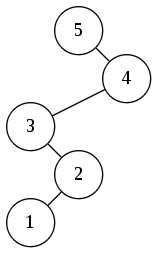
\includegraphics[width=0.22\textwidth]{Grafos/ej3figura1.png}
% \hspace{100pt}
%  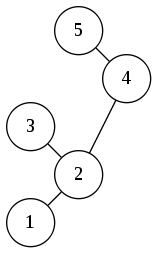
\includegraphics[width=0.22\textwidth]{Grafos/ej3figura2.png}
% \begin{center}
%  Grafo $T$ \hspace{160pt} Grafo $S$
% \end{center}
% \end{center}

En el ejemplo mostrado $e$ ser\'ia la arista (3,4) y $e'$ ser\'ia (2,4). Sea $S'=S+e-e'$, de esta manera $S'$ es \'arbol generador de $G$. Si $l(e')<l(e)$ ($l(e)=$ peso de la arista $e$) llego a un absurdo. Esto se puede ver porque $S$ contiene todas las aristas anteriores a $e$ m\'as $e'$ y no se forma un ciclo en dicho grafo, por consiguente el algoritmo que va armando el grafo $T$ hubiese elegido a $e'$ en lugar de $e$ y esto es absurdo porque dijimos que $e'$ no pertenece a $T$. Entonces tenemos que $l(e')\geq l(e)$. Podemos apreciar entonces que el peso de $S'$ es a lo sumo igual al de $S$, pero no puede ser menor porque $S$ es AGM. Esto implica que $S'$ tiene el mismo peso que $S$ y entonces tambien es \'arbol generador m\'inimo de $G$ (conteniendo las aristas prefijadas), m\'as a\'un, $S'$ tiene una arista m\'as en com\'un con $T$ que $S$. Repitiendo este paso para todas las aristas distintas entre $T$ y $S$ (como m\'aximo ser\'an $l-f-1$ pasos, donde $l$ es la cantidad de nodos y $f$ la cantidad de pares fijados por Astor), se llegar\'a a un grafo \'arbol generador m\'inimo de $G$ con las mismas aristas de $T$, lo que es absurdo porque partimos de que $T$ no es m\'inimo.

\end{itemize}

\section*{Complejidad}

Para calcular la complejidad de este ejercicio el modelo utilizado fue el uniforme, esto se debe a que lo que define el orden del algoritmo es la cantidad de nodos y de aristas (y cómo están relacionados los nodos  por dichas aristas). Es decir, no es relevante observar el tamaño que ocupa cada nodo, sino la cantidad de nodos que contenga el grafo. En consecuencia, la utilizaci\'on del modelo logaritm\'ico carece de sentido para este tipo de problema.

Antes de comenzar, es importante aclarar lo siguiente: Al contar con un grafo completo como parámetro de entrada, el mismo posee $n*(n-1)$ aristas, siendo $n$ la cantidad de nodos. Es decir que $O(n^2) = O(m)$, por lo que, de ahora en adelante, consideraremos a $n$ como único parámetro al calcular la complejidad.

A continuación analizaremos parte por parte la complejidad de cada función del algoritmo:

\begin{verbatim}
  aristasPorAgregar = lista de aristas del grafo original
  aristasAstor = lista de aristas prefijadas por Astor
\end{verbatim}

El primer paso de la función principal consiste en crear dos listas donde se almacenarán aristas. Para la primera se cuenta con $m = n*(n-1)$ aristas mientras que para la segunda, la cantidad de aristas será menor ya que las aristas fijadas no pueden superar a $n-1$ (porque sino habría ciclos y el problema no tendría solución). Por lo tanto hasta aquí la complejidad resulta de orden $O(n^2)$.

\begin{verbatim}
  ordenar aristasPorAgregar por peso
\end{verbatim}

Como se mencionó antes, el algoritmo utilizado para realizar el ordenamiento es una variante del \textit{Mergesort} optimizada, por lo que su complejidad es $O(m*log(m)) = O(n^2*log(n^2)) = O(n^2*log(n))$.

\begin{verbatim}
  insertar aristasAstor en el grafo resultado
  costoProduccion = sumo los pesos de todas las aristas de astor
\end{verbatim}

La primera operación de inserción resulta $O(n)$ por la cota vista, por la que las aristas de Astor no pueden ser más de $n-1$. Con respecto a la segunda operación, es del mismo orden por la misma causa.

\begin{verbatim}
  mientras la cantidad agregada sea menor a n-1 nodos
    tomo una arista de aristasPorAgregar
    si se puede insertar la arista (sePuedeMeter)
      sumar a costoProduccion el peso de la arista
      insertar la arista en el grafo resultado (meterArista)
\end{verbatim}

En esta parte, hay un ciclo que se realiza como máximo, $m$ cantidad de veces, debido a que en el peor caso se recorrerán las $m$ aristas del grafo completo. Esto se debe a que en cada iteración una determinada arista es insertada en el grafo resultado, o es descartada como posible arista a insertar.

Con respecto a las operaciones realizadas dentro del ciclo, la primera resulta constante porque consiste en tomar el primer elemento de una lista enlazada. Luego se verifica si la arista obtenida se puede insertar llamando a la funcion \textit{sePuedeMeter()}. Esta función tiene un costo de peor caso $O(1)$ como veremos más adelante. En caso de poder meter la arista, se realizan dos operaciones: Una suma de costo constante y la insercion de la arista en el grafo. Del mismo modo, veremos luego que la complejidad de esta última función es $O(n)$.

A partir de lo mencionado anteriormente, podemos concluir que la complejidad total de este fragmento del algoritmo resulta $O(n*m) = O(n^3)$ ya que la operación de mayor costo dentro del ciclo es lineal con respecto a $n$ y la cantidad de iteraciones es a lo sumo $O(n^2)$.

\begin{verbatim}
  ordenar las aristas del grafo resultado segun los valores de los nodos
\end{verbatim}

Al igual que antes, \textit{Mergesort} realizará esta operación en $O(n*log(n))$ ya que el grafo resultado posee $n-1$ aristas por ser árbol generador del grafo original.

\bigskip
Por todo esto, podemos afirmar que la complejidad total del algoritmo es $O(n^3)$ ya que ninguna parte del algorimo supera la complejidad del ciclo analizado.

\subsection*{sePuedeMeter()}

\begin{verbatim}
si los dos nodos pertenecen a distintas componentes conexas
o si alguno de los dos no pertenece a ninguna
  retornar true
sino
  retornar false
\end{verbatim}

Como vimos anteriormente, verficar esta condición implica el acceso a dos posiciones de cada arreglo (\textit{índices} y \textit{componentesConexas}) por lo cual el orden resulta $O(1)$.

\subsection*{meterArista()}

\begin{verbatim}
si ninguno de los dos nodos pertenece a alguna componente conexa
  asignar una nueva componente conexa a ambos nodos

sino si un nodo pertenece a alguna componente y el otro no
  asignar al otro nodo esa componente

sino si ambos nodos pertenecen a componentes conexas distintas
  uno las dos componentes en una y le asigno a ambos nodos esa componente

agrego la arista al grafo resultante
\end{verbatim}

La primer etapa de la función consiste en evaluar los 3 casos mencionados anteriormente en la descripción del algoritmo. Para los primeros dos, se realizan únicamente operaciones en una cantidad de posiciones acotadas de ambos arreglos por lo cual la complejidad es constante. Sin embargo, el último caso, encargado de unir las dos componentes conexas es $O(n)$ en el peor caso, ya que se deberá recorrer el arreglo de tamaño $n$ para cambiar las posiciones de los nodos relativos a una de las dos componentes conexas. Con respecto a la última operación, es trivial observar que dicho costo es de orden constante ya que se trata de agregar un elemento a una lista enlazada.

Por todo esto, podemos concluir que la función meterArista() es $O(n)$ para el peor caso.

\bigskip

Finalmente estudiaremos la complejidad en funci\'on del tama\~{n}o de la entrada. Sea $t$ el tama\~{n}o de la entrada, $n$ la cantidad de locales, $f$ la cantidad de aristas de Astor, $L$ la matriz de pesos de las aristas y $F$ el arreglo de aristas de Astor. Tenemos entonces que:

$$t=\log(n)+\log(f)+\sum_{i=1}^{n}\sum_{j=1}^{n}\log(L_{i,j})+\sum_{i=1}^{f}\log(F_{i})>\log(n)+\log(n)+\sum_{i=1}^{n}\sum_{j=1}^{n}1+\sum_{i=1}^{f}1>2\log(n)+n^{2}+n>n^{2}$$

\hspace{45pt} $\Longrightarrow$ como $T(n) \in O(n^{3})$ y $n^{3}=(n^{2})^{3/2}<t^{3/2} \Longrightarrow T(t) \in O(t^{3/2})$

\section*{An\'alisis de resultados}

En la siguiente secci\'on analizaremos el comportamiento en la pr\'actica del algoritmo propuesto. El an\'alisis est\'a basado en estudiar el tiempo de ejecuci\'on para instancias aleatorias en funci\'on de la cantidad de locales manteniendo fija la cantidad de pares de locales fijados por Astor es decir, seg\'un el modelo propuesto, la cantidad de aristas a ingresar en el \'arbol antes de iniciar el algoritmo. A su vez, se ver\'a la relaci\'on que existe entre la complejidad te\'orica calculada y los resultados obtenidos. Adem\'as, para completar el an\'alisis se estudiar\'an los peores casos que presenta el algoritmo.

Para realizar los tiempos de ejecuci\'on, se implement\'o un algoritmo que genera instancias aleatorias, es decir, genera la matriz de los pesos de cada arista para todo el grafo completo y una cierta cantidad de aristas, que representan los locales fijados por Astor, asegur\'andose que no formen un ciclo.

A continuaci\'on se presentan los resultados de las pruebas realizadas para instancias aleatorias, variando la cantidad de locales y manteniendo fija la cantidad de pares fijado por Astor en $4$, $20$ y $50$.

% \begin{center}
%  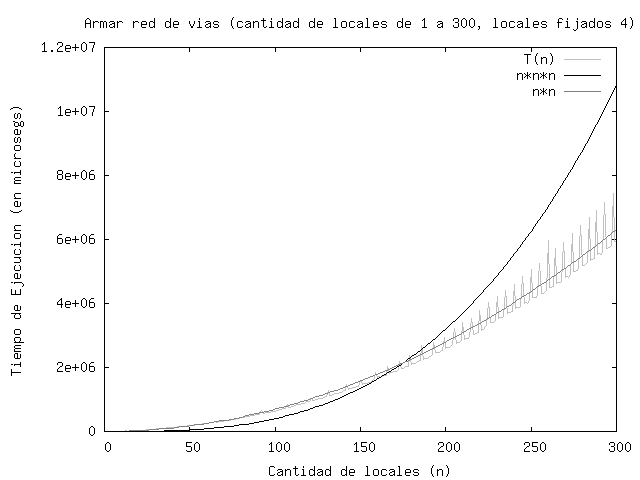
\includegraphics[width=0.7\textwidth]{Plots/Tp2Ej3-Complejidad.png}
% \begin{center}
% Figura 3.1
% \end{center}
% \end{center}
% 
% \begin{center}
%  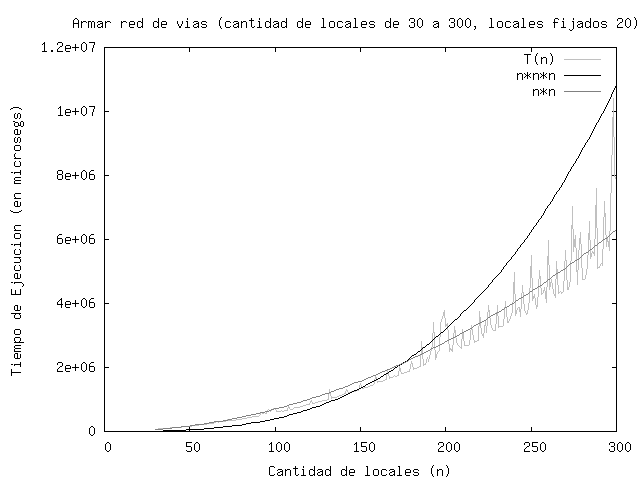
\includegraphics[width=0.7\textwidth]{Plots/Tp2Ej3-Complejidad-20.png}
% \begin{center}
% Figura 3.2
% \end{center}
% \end{center}
% 
% \begin{center}
%  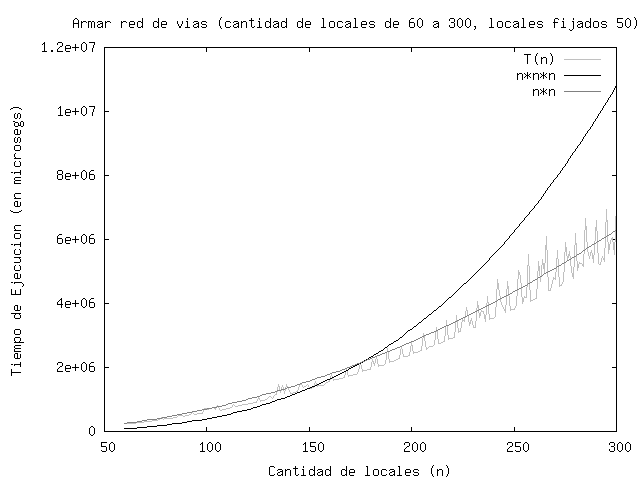
\includegraphics[width=0.7\textwidth]{Plots/Tp2Ej3-Complejidad-50.png}
% \begin{center}
% Figura 3.3
% \end{center}
% \end{center}

Como se puede apreciar, en las figuras $3.1$, $3.2$ y $3.3$ el crecimiento de la funci\'on que mide el tiempo de ejercuci\'on es similar, a pesar de que, a mayor cantidad de locales fijados por Astor, los tiempos se vuelven m\'as irregulares. La similitud en el crecimiento de los gr\'aficos se debe a que el tiempo que tarda algoritmo depende sobre todo de la disposici\'on de las aristas fijadas por Astor y de la forma en que se van agregando las aristas durante el algoritmo de Kruskal, y no tanto de la cantidad de aristas recibidas. Es decir, si se mantiene fija la cantidad de aristas de Astor y se aumenta significativamente la cantidad de locales totales, la incidencia de este par\'ametro en el tiempo de ejecuci\'on ser\'a m\'inima.

Es importante observar que en las figuras presentadas el crecimiento de la funci\'on del tiempo de ejecuci\'on es menor que la cota te\'orica propuesta, $O(n^{3})$. El gr\'afico muestra adem\'as que dicho crecimiento se asemeja mucho m\'as al orden cuadr\'atico. Esto se debe a la forma en que el algoritmo arma el \'arbol resultante: la mayor\'ia de las aristas que agrega en los sucesivos pasos del algoritmo de Kruskal, se agregan en tiempo constante. Agregar una arista es de orden lineal s\'olo en el caso en que dicha arista une dos componentes conexas del \'arbol, es decir, cuando se deben recorrer las estructuras utilizadas para cambiar una de las componentes conexas fusionadas. Sin embargo, emp\'iricamente esta \'ultima operaci\'on  se realiza pocas veces en relaci\'on a la cantidad total de aristas agregadas. Por esta raz\'on, en el caso promedio la complejidad del algoritmo es menor que la cota te\'orica propuesta de $O(n^{3})$. Por medio de las pruebas, podr\'iamos afirmar entonces que en la pr\'actica el algoritmo presentado se asemeja m\'as a un algoritmo de orden cuadr\'atico que a uno c\'ubico.

Seg\'un lo mencionado anteriormente, se puede deducir que los peores casos ser\'an aquellos en los que agregar una arista al \'arbol resultado implique unir componentes conexas y, por lo tanto, tener que cambiar la estructura que guarda el n\'umero de componente conexa de cada nodo (llamada ComponentesConexas en la secci\'on ``Algoritmo``). A continuaci\'on presentaremos un ejemplo de peor caso y lo explicaremos en detalle.

% \begin{center}
%  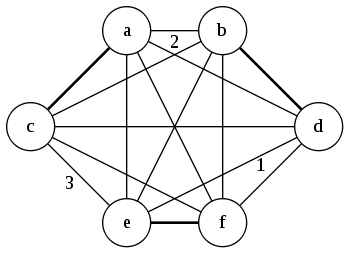
\includegraphics[width=0.6\textwidth]{Grafos/ej3peorcaso.png}
% \begin{center}
% Figura 3.4
% \end{center}
% \end{center}

En primer lugar, se deben hacer ciertas aclaraciones: 
\begin{itemize}
 \item Las aristas fijadas por Astor son las que figuran resaltadas.
 \item El peso de las aristas del ''interior del grafo'' es mayor que las del ``borde``.
\end{itemize}

Como se puede notar en el gr\'afico, la arista de menor peso es la $D-F$ por lo que ser\'a la primera en ser agregada en el algoritmo. Agregar esta arista implica unir las componentes conexas de las aristas $E-F$ y $D-B$, por lo que se deber\'a recorrer todo el arreglo ComponentesConexas para eliminar las apariciones de la componente conexa $D-B$ y as\'i fusionar las tres aristas mencionadas en una \'unica componente conexa que contenga a los nodos E, F, D, B. Esta misma operaci\'on se realizar\'a para unir esta \'ultima componente conexa con la componente que contiene a los nodos C y A por medio de la arista $A-B$. En este caso, todas las aristas agregadas unieron componentes conexas, por lo que se debi\'o recorrer el arreglo ComponentesConexas por cada arista haciendo que este sea un peor caso para el algoritmo presentado. Cabe aclarar que estos casos dependen tanto de la disposici\'on tanto de las aristas de Astor, como del peso de las aristas a agregar. Esto hace que generar peores casos para estudiar el tiempo de ejecuci\'on sea d\'ificil. Sin embargo, seg\'un el ejemplo presentado y la cota te\'orica propuesta se puede apreciar que el tiempo de los peores casos ser\'a del orden de $n^{3}$.

\section*{Conclusiones}

A partir de las secciones detalladas anteriormente se pueden realizar las siguientes conclusiones y aclaraciones. En primer lugar, es importante aclarar que a la hora de resolver el problema se podr\'ian haber utilizado otro tipo de estructuras para mejorar el rendimiento del algoritmo. Como el algoritmo propuesto se basa principalmente en hacer operaciones de bu\'squeda y uni\'on sobre distintos conjuntos de nodos, se podr\'ia haber utilizado una estructura \textit{Union-Find}\footnotemark[1]. En la pr\'actica este tipo de estructuras hacen que el algoritmo mejore significativamente su complejidad debido a que las operaciones de uni\'on y b\'usqueda son pr\'acticamente lineales (utilizando algoritmos inteligentes sobre listas y \'arboles). Cabe aclarar que a pesar de esto la cota te\'orica es la misma que se obtiene con las estructuras utilizadas en nuestro algoritmo.

Como se pudo observar emp\'iricamente, llegamos a la conclusi\'on de que el algoritmo es mejor en promedio de lo que se esperaba en teor\'ia. Es decir, se mostr\'o que tiene un comportamiento del orden cuadr\'atico para la mayor\'ia de los casos, aunque existen casos en lo que esto no es cierto. Cabe mencionar tambi\'en que se podr\'ian haber hecho otras pruebas para estudiar el comportamiento del algoritmo. En concreto, se podr\'ia haber hecho un an\'alisis de los tiempos de ejecuci\'on en funci\'on de la cantidad de aristas de Astor, manteniendo fija la cantidad de locales. Se supone que a medida que aumente la cantidad de aristas de Astor para una cantidad de locales fija, el tiempo de ejecuci\'on deber\'ia disminuir ya que debe agregar menor cantidad de aristas teniendo que chequear si se forma un ciclo.

Finalmente, podemos concluir que el problema podr\'ia haber sido resuelto de manera un poco m\'as eficiente de haber tenido tiempo adicional. Sin embargo, en la pr\'actica, el tiempo de ejecuci\'on del algoritmo propuesto se asemeja m\'as al de los algoritmos que utilizan \textit{Union-Find} que a un algoritmo de orden c\'ubico.

\footnotetext[1]{Ver referencias sobre este tipo de estructuras en la secci\'on ''Referencias''}

\section*{Referencias}
\begin{itemize}
 \item Art\'iculo de Wikipedia sobre Programaci\'on Din\'amica
 \item Art\'iculo de Wikipedia sobre Grafos
 \item Art\'iculo de Wikipedia sobre Algoritmo de Kruskal
 \item Art\'iculo de Wikipedia sobre Estructuras Union-Find
 \item Art\'iculo de Wikipedia sobre Depth/Breadth First Search
\end{itemize}


\end{document}
